\documentclass[]{article}
\usepackage{lmodern}
\usepackage{amssymb,amsmath}
\usepackage{ifxetex,ifluatex}
\usepackage{fixltx2e} % provides \textsubscript
\ifnum 0\ifxetex 1\fi\ifluatex 1\fi=0 % if pdftex
  \usepackage[T1]{fontenc}
  \usepackage[utf8]{inputenc}
\else % if luatex or xelatex
  \ifxetex
    \usepackage{mathspec}
  \else
    \usepackage{fontspec}
  \fi
  \defaultfontfeatures{Ligatures=TeX,Scale=MatchLowercase}
\fi
% use upquote if available, for straight quotes in verbatim environments
\IfFileExists{upquote.sty}{\usepackage{upquote}}{}
% use microtype if available
\IfFileExists{microtype.sty}{%
\usepackage{microtype}
\UseMicrotypeSet[protrusion]{basicmath} % disable protrusion for tt fonts
}{}
\usepackage[margin=1in]{geometry}
\usepackage{hyperref}
\hypersetup{unicode=true,
            pdftitle={2 VLSM: Vector-based Landscape Metrics in QGIS},
            pdfborder={0 0 0},
            breaklinks=true}
\urlstyle{same}  % don't use monospace font for urls
\usepackage{graphicx,grffile}
\makeatletter
\def\maxwidth{\ifdim\Gin@nat@width>\linewidth\linewidth\else\Gin@nat@width\fi}
\def\maxheight{\ifdim\Gin@nat@height>\textheight\textheight\else\Gin@nat@height\fi}
\makeatother
% Scale images if necessary, so that they will not overflow the page
% margins by default, and it is still possible to overwrite the defaults
% using explicit options in \includegraphics[width, height, ...]{}
\setkeys{Gin}{width=\maxwidth,height=\maxheight,keepaspectratio}
\IfFileExists{parskip.sty}{%
\usepackage{parskip}
}{% else
\setlength{\parindent}{0pt}
\setlength{\parskip}{6pt plus 2pt minus 1pt}
}
\setlength{\emergencystretch}{3em}  % prevent overfull lines
\providecommand{\tightlist}{%
  \setlength{\itemsep}{0pt}\setlength{\parskip}{0pt}}
\setcounter{secnumdepth}{0}
% Redefines (sub)paragraphs to behave more like sections
\ifx\paragraph\undefined\else
\let\oldparagraph\paragraph
\renewcommand{\paragraph}[1]{\oldparagraph{#1}\mbox{}}
\fi
\ifx\subparagraph\undefined\else
\let\oldsubparagraph\subparagraph
\renewcommand{\subparagraph}[1]{\oldsubparagraph{#1}\mbox{}}
\fi

%%% Use protect on footnotes to avoid problems with footnotes in titles
\let\rmarkdownfootnote\footnote%
\def\footnote{\protect\rmarkdownfootnote}

%%% Change title format to be more compact
\usepackage{titling}

% Create subtitle command for use in maketitle
\providecommand{\subtitle}[1]{
  \posttitle{
    \begin{center}\large#1\end{center}
    }
}

\setlength{\droptitle}{-2em}

  \title{2 VLSM: Vector-based Landscape Metrics in QGIS}
    \pretitle{\vspace{\droptitle}\centering\huge}
  \posttitle{\par}
    \author{}
    \preauthor{}\postauthor{}
      \predate{\centering\large\emph}
  \postdate{\par}
    \date{2019-08-26}

\usepackage{float}

\begin{document}
\maketitle

\section{1 Vignette Info}\label{vignette-info}

Most common landscape metrics are calculated on a raster-basis. However,
sometimes landscape information come along in vector-formats. For the
calculation of landscape metrics, one must perform a
vector-to-raster-transformation often resulting in a loss of
information. In \textbf{VLSM} we implemented various landscape metrics
based on vector data in \texttt{R}. However, sometimes it is easier to
process data with only few clicks using a desktop GIS. Therefore, we
created compatible R scripts being accessible in the open-source desktop
GIS \texttt{QGIS}. In the following, a quick manual on how to use these
functions in \texttt{QGIS}. If you want to use these functions via
\texttt{R}, please refer to
\href{https://github.com/raff-k/VLSM/blob/master/vignettes/vignette_R.pdf}{here}.

\section{2 Packages and Software
Utilities}\label{packages-and-software-utilities}

The open-source desktop GIS \texttt{QGIS} enabele the possibility to
integrate R-scripts. However, \texttt{QGIS} does not except the standard
\texttt{.R}-format, instead we developped R-scripts which are
compartible to \texttt{QGIS} and can easily be loaded in with only few
clicks. You can find the \textbf{VLSM} R-scripts for \texttt{QGIS}
\href{https://github.com/raff-k/VLSM/blob/master/R_QGIS}{here}.

We tested our implementation on Windows with the following software and
packages: * Before integrating \texttt{R} into \texttt{QGIS}, one must
have installed \texttt{R}
(\href{https://cran.r-project.org/}{download-page}). Our implementation
was tested using \emph{R version 3.5.2 (2018-12-20) -- ``Eggshell
Igloo''}. Furthermore, we recommend to install the necessairy packages
\href{https://cran.r-project.org/web/packages/sf/index.html}{sf},
\href{https://cran.r-project.org/web/packages/sp/index.html}{sp},
\href{https://cran.r-project.org/web/packages/raster/index.html}{raster},
\href{https://cran.r-project.org/web/packages/link2GI/index.html}{link2GI},
\href{https://cran.r-project.org/web/packages/rgrass7/index.html}{rgrass7},
\href{https://cran.r-project.org/web/packages/RSAGA/index.html}{RSAGA},
\href{https://cran.r-project.org/web/packages/dplyr/index.html}{dplyr},
and of course \href{https://github.com/raff-k/VLSM}{VLSM} via
\texttt{R}. * \textbf{QGIS 3.6 Noosa}: We recommend
\texttt{QGIS}\textgreater{} 3.x which can easily be installed by the
\href{https://live.osgeo.org/de/download.html}{OSGeo-installer}. In
\texttt{QGIS} one must enable the option for R-processing, first. An
comprehensive instruction can be found
\href{https://docs.qgis.org/3.4/en/docs/training_manual/processing/r_intro.html}{here},
or
\href{https://gis.stackexchange.com/questions/273623/r-scripts-in-qgis-3-0}{here}.
It may be that \texttt{R} is not visible or included in the setting
menu. If that is the case the \texttt{Processing\ R\ Provider} must
installed as plug-in (see
\href{https://gis.stackexchange.com/questions/273623/r-scripts-in-qgis-3-0}{here}
for help).

\emph{Note:} One can set \texttt{R\textquotesingle{}s} library directory
in QGIS. Installing necessairy packages may be better done inside
\texttt{R}.

When the setup of the setting was successfull, the \texttt{QGIS} desktop
should look similiar to the following screenshot:

\begin{figure}[H]

{\centering 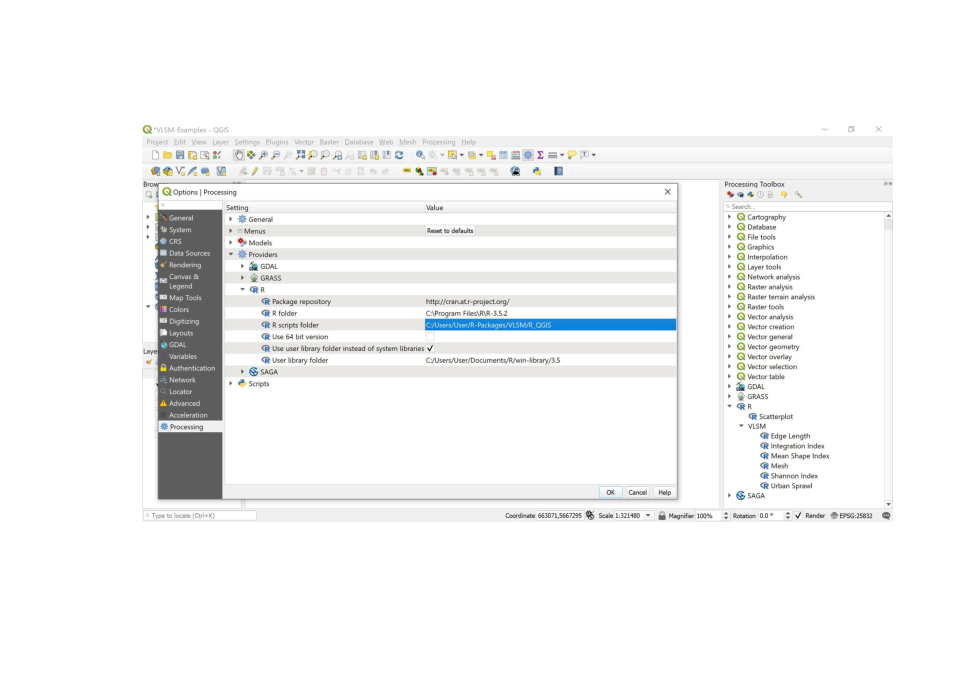
\includegraphics[width=1\linewidth]{vignette_QGIS_files/figure-latex/unnamed-chunk-2-1} 

}

\caption{QGIS setting to access R functions}\label{fig:unnamed-chunk-2}
\end{figure}

\section{3 Calculation of Landscape
Metrics}\label{calculation-of-landscape-metrics}

We use Corine Land Cover (CLC) data, which are in detailed explained in
the
\href{https://github.com/raff-k/VLSM/blob/master/vignettes/vignette_R.pdf}{R-vignette}
of this package.

\subsection{3.1 Example 1: Effective Mesh
Size}\label{example-1-effective-mesh-size}

The \emph{effective mesh size} is calculated with the tool \emph{Mesh}.
The output delivers a table with the corresponding mesh sizes {[}ha{]}.

\begin{figure}[H]

{\centering 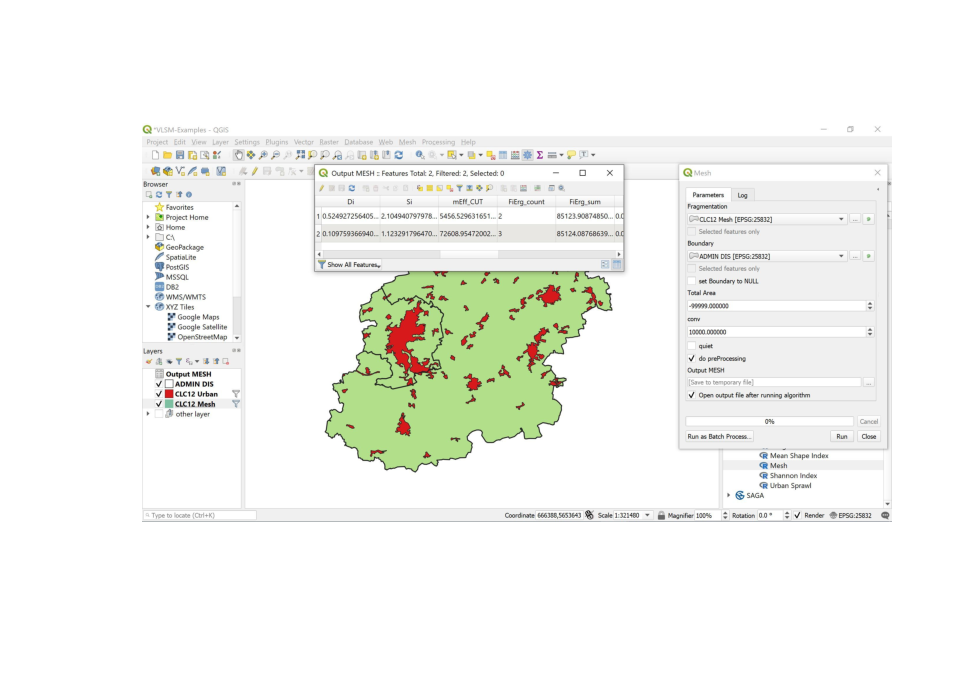
\includegraphics[width=1\linewidth]{vignette_QGIS_files/figure-latex/unnamed-chunk-3-1} 

}

\caption{Calculation of Effective Mesh Size in QGIS}\label{fig:unnamed-chunk-3}
\end{figure}

\subsection{3.2 Example 2: Urban Sprawl}\label{example-2-urban-sprawl}

The \emph{Urban Sprawl} is calculated with the tool \emph{Urban Sprawl}.
The output delivers a table with the corresponding degree of urban
sprawl {[}\%{]}, and a geometry showing the grid lines, which were used
for calculation.

\begin{figure}[H]

{\centering 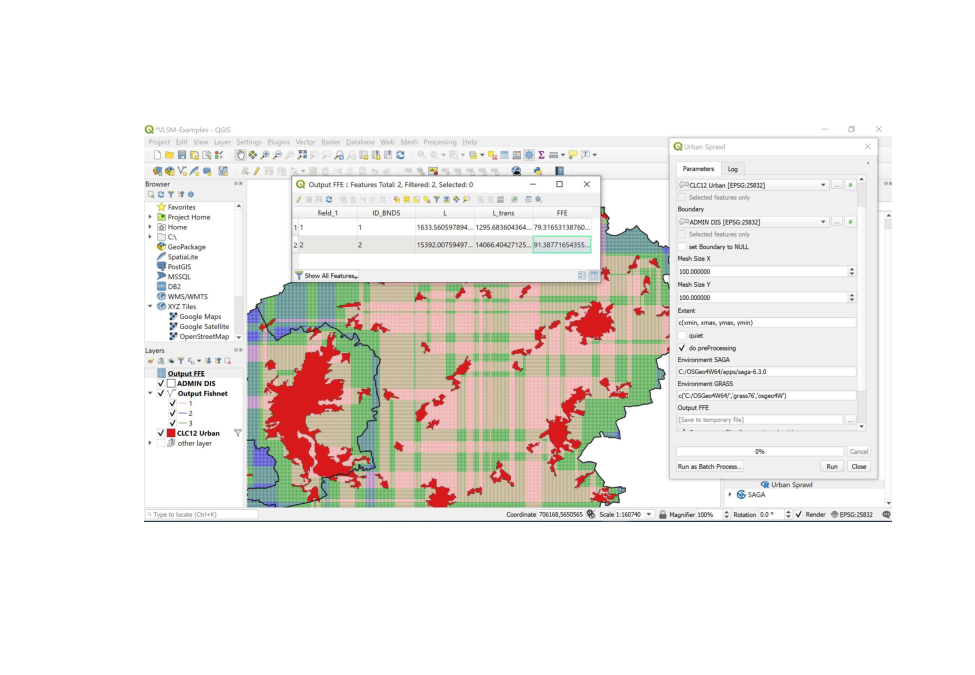
\includegraphics[width=1\linewidth]{vignette_QGIS_files/figure-latex/unnamed-chunk-4-1} 

}

\caption{Calculation of Urban Sprawl in QGIS}\label{fig:unnamed-chunk-4}
\end{figure}


\end{document}
